%% ------------------------------------------------------------------------- %%
\chapter{Avaliação}
\label{cap:avaliacao}


\section{Implantando coreografias com e sem o EE}

In this section, we assess how
the \choreos \ee improves the deployment process by providing a middleware-supported solution.
We conducted this assessment by developing an \emph{ad-hoc} solution
dedicated to the deployment of a single choreography.
The ``Airport choreography'' is an example provided by Airport domain
experts~\cite{Choreos2012D6.2} containing 15 services.
We also deployed the same choreography using the \ee.
Both solutions are publicly available.
% link pro adhoc

To deploy the Airport choreography with the \ee, we wrote the choreography
specification and a program to invoke the \ee, launching the deployment.
The choreography specification was assembled with simple Java objects consisting of 162 lines,
with 11 lines of code per service on average.
The code was written in the \texttt{AirportSpecs} class in 40 minutes.
The deployment launch program, \texttt{AirportEnact} class, uses the \ee Java API and has only 22 lines of code.
After this code was written, deploying the choreography over three nodes with \ee
took only 4 minutes.

To develop the \emph{ad-hoc} solution, it was necessary nearly 9 hours of one programmer,
and additional 60 minutes to execute the deployment, using the same programmer, 
distributing the 15 services over three different nodes. 
This solution required the writing of
100 LoC of shell scripts, 220 LoC of Java, and 85 LoC of Ruby (for Chef). 

In the remaining of this section, we describe the process of creating and executing
the \emph{ad-hoc} deployment solution. We highlight the difficulties in the process
that the deployer must face without the \ee usage.

The deployment of each service is executed by a Chef recipe within a cookbook.
We wrote one cookbook template, to deploy JAR services,
and we used it to generate the cookbooks for the 15 participant services.
The process of creating the 15 cookbooks was partially automated by
the \texttt{generate} script that we wrote.
The service package URLs had to be manually inserted on cookbooks
after running the \texttt{generate} script.

To implement service binding,
we developed a small but no trivial Java program, called \texttt{context\_sender}. 
It is responsible for invoking the \texttt{setInvocationAddress} operation of a given service.
We implemented \texttt{context\_sender} as a Java program to take advantage of
the SOAP API provided by the Java SE environment.
We also developed the \texttt{bind\_services} script,
responsible for calling \texttt{context\_sender} for each dependency within the choreography.
Since service IP addresses are known only after deployment, the \texttt{bind\_services}
is actually a template with some tokens that must be replaced with the deployed services IPs.

The execution of the \emph{ad-hoc solution} has several steps, including some manual ones. 
For each target node, the deployer must log into it, install git, 
checkout the cookbooks, execute the \texttt{install\_chef} script, 
edit some configuration files defining which services will be deployed on the node,
and run chef-solo. 
After deploying the services, the deployer must edit the IP tokens
within the \texttt{bind\_services} script,
and finally execute the \texttt{bind\_services} script.
Some overall problems of this \emph{ad-hoc} solution are:

\begin{itemize}

\item Three different technologies:
shell script, Java and Chef.
Command line expertise was also necessary at some steps,
like using the vim editor or using the \texttt{ps} command
to verify service processes.
It suggests that it requires a large set of skills 
from the implementor of deployment solutions.
Some of this skills, such as using Chef, are known not to be easy to learn.
The Java code used to invoke SOAP services may also be considered as
non-trivial for a programmer not used to this technology.

\item Code duplication on the generated cookbooks.
If something changes on the template, it is necessary to regenerate all cookbooks,
performing the required manual edition, too.
However, we acknowledge that the above mentioned manual editions 
could be avoided with some more complex scripting.
Code replication could  also be avoided by creating a ``Chef LWRP'',
but this would be a task to advanced users of Chef.

\item For each target node, the deployer must perform time-consuming manual steps.
Some (e.g., executing \texttt{install\_chef}) could be avoided
by using a tool like Capistrano\footnote{\url{http://www.capistranorb.com/}}, 
but it would require one more technology to be learned.
Other manual steps, like editing configuration files, are very error-prone.
Missing commas or mistyping service names are likely to happen.

\item There are very little concurrency in the process. 
With the provided scripts, the deployer could somehow enhance parallelism
by using tools like Byobu\footnote{\url{http://byobu.co/}} 
to enter the same command in multiple machines.
But this requires yet another ability from the deployer 
and it is still a limited way to scale the process.

\end{itemize}

Note that, in this example, we used a service composition with only 15 services.
Using large-scale compositions would increase much more
the complexity of the \emph{ad-hoc} solution.
To reach a complete solution in the \emph{ad-hoc} approach, 
an extra development effort would be required 
to implement features already provided by the \ee,
such as third-party failure handling,
composition update, dynamic node allocation policies,
concurrent deployment, etc.
In addition, to produce the \emph{ad-hoc} solution we used some code already 
available in the \ee, such as the cookbook template and
the \texttt{context\_sender}. Deployers would have to code them from scratch.

We must recognize that this assessment by comparison with an \emph{ad-hoc} solution 
has its limitations,
since results depend strongly on the deployer's technical skills.
Conducting a rigorous software engineering experiment with several developers
assuming the deployer's role would bring a stronger evidence.
However, we believe that the assessment described here is enough for 
expanding our understanding of the value added by a middleware-supported
solution such as the \choreos \ee as it provides a good illustration
of the effort required to deploy such systems.

\section{Análise de desempenho e escalabilidade}

We conducted experiments to evaluate the performance and scalability of
the proposed \ee in terms of its capability to deploy a significant number of
compositions in a real-world cloud computing platform.

Our experiments use a synthetic workload modeled
as depicted in Figure~\ref{fig:eval_composition}.
The arrow direction is from the requester to the requested service.
Although replies are not drawn for simplicity reasons, they are always sent back
in a synchronous manner.
This topology was chosen because (1) it is a representative example of the most common business process (those composed by branches -- calls to other systems -- and subsequent joints) and (2) it follows a repetitive pattern that can be used to smoothly increase the size of the composition to analyze how the performance of the \ee behaves as its workload increases.

\begin{figure}[h]
  \centering
  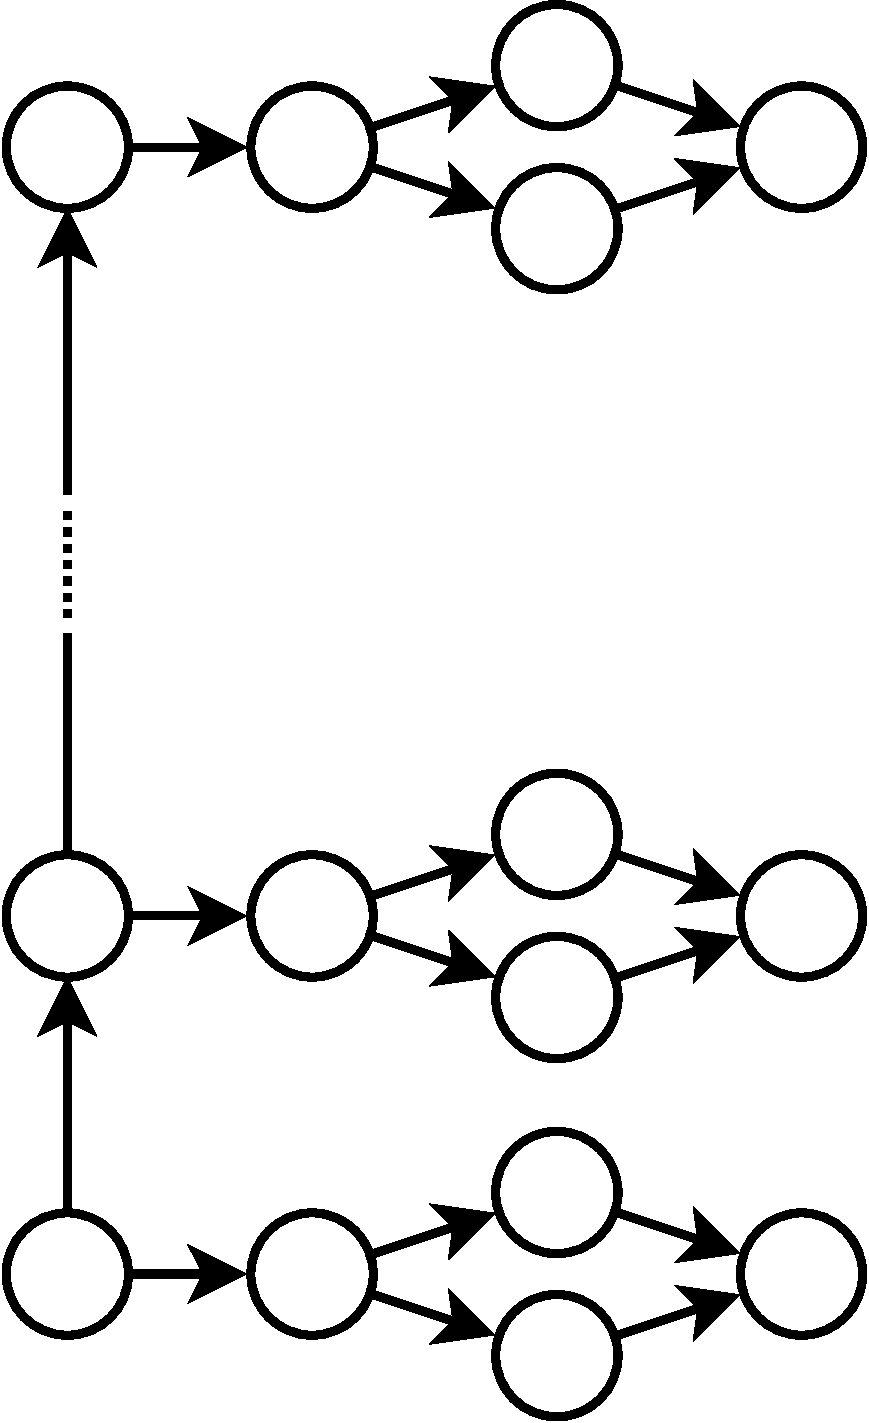
\includegraphics[width=.3\linewidth, angle=270]{eval_composition.pdf}
  \caption{The topology of the compositions used in the experiments.}
  \label{fig:eval_composition}
\end{figure}


Initially, we conducted a multi-variable analysis of the \ee performance by deploying service compositions
in the following scenarios:
1) a small set of small compositions;
2) a small set of larger compositions;
3) a larger set of small composition;
4) a larger ratio of services per node.
Table~\ref{tab:cases} quantifies each scenario.

\begin{table}
\centering
\caption{Deployment scenario in the experiments}
\label{tab:cases}
\begin{tabular}{c c c c c} \hline
\emph{Scenario} & \emph{Compositions} & \emph{Size} & \emph{Nodes} & \emph{Serv/Node} \\ \hline
1 &  10 &  10 &  9 & 11 or 12 \\
2 &  10 & 100 & 90 & 11 or 12 \\
3 & 100 &  10 & 90 & 11 or 12 \\
4 &  10 &  10 &  5 &       20 \\
\hline \end{tabular}
\end{table}

In our experiments, 
the node allocation policy was ``limited round robin'',
in which services are distributed across the available nodes,
and the quantity of nodes is configured before each experiment.
If the amount of services is not divisible by the number of nodes,
some nodes will host one additional service.
The idle node reservoir size was five,
and the node creation timeout was 300 seconds.
We used Amazon EC2
as the cloud computing service and the VMs were EC2 small instances,
each one with 1.7 GiB of RAM, one vCPU
with processing power equivalent to 1.0--1.2 GHz,
and running Ubuntu GNU/Linux 12.04.
The \ee was executed on a machine with 8 GB of
RAM, an Intel Core i7 CPU with 2.7 GHz and GNU/Linux kernel 3.6.7.
The \ee version used for the experiments
and raw data retrieved from executions
are available online\footnote{\url{http://ccsl.ime.usp.br/enactmentengine}} for reproducibility of the results.

Each scenario was executed 30 times
and the Table~\ref{tab:results} presents, for each scenario,
the time necessary to deploy all compositions
plus the time to invoke them to make sure they were correctly deployed.
The values are averages with 95\% confidence intervals.
It also shows how many compositions and services were successfully deployed.

\begin{table}
\centering
\caption{Experimental results}
\label{tab:results}
\begin{tabular}{c r@{ $\pm$ }l r@{ $\pm$ }l r@{ $\pm$ }l} \hline

\emph{Scenario} & \multicolumn{2}{c}{\emph{Time}} & \multicolumn{2}{c}{\emph{Successful}}   & \multicolumn{2}{c}{\emph{Successful}}\\
                 & \multicolumn{2}{c}{}           & \multicolumn{2}{c}{\emph{Compositions}} & \multicolumn{2}{c}{\emph{Services}}\\
\hline
1 &  467.9 &  34.8 & 10.0 & 0   & 100.0 & 0   (100\%) \\
2 & 1477.1 & 130.0 &  9.3 & 0.3 & 999.3 & 0.4 (99.9\%)\\
3 & 1455.2 & 159.1 & 98.9 & 0.8 & 998.5 & 1.3 (99.9\%)\\
4 &  585.2 &  38.1 & 10.0 & 0.1 & 100.0 & 0.1 (100\%)\\
\hline \end{tabular}
\end{table}

The results show that the \ee scales well in terms of the number of
services being deployed. Although the number of services was
multiplied by 10, the deployed time increased only 3 times approximately
in scenarios 2 and 3.
This time increment was caused mainly by the fact that
the higher the number of services, the higher the likelihood
of a fault triggering the re-execution of some routine.

The results also show that when the number of services per node was doubled (scenario 4),
the deployment time increased nearly 25\%. Part of this overhead was caused by
the increase on the number of Chef scripts that must be executed (sequentially)
on the nodes.

During our experiments, we observed that, thanks to the \ee fault tolerance mechanisms, the amount of failures was
low: all the services were successfully deployed in more than 75\% of the executions.
By a failure, we mean that one service was not properly deployed.
In scenario 1 we got no failures, 
whereas in scenario 4 we had only one failure.
In scenario 2, the worst situation was 3 failures out of 1,000 services.
In scenario 3, we got one execution with 20 failures, but it was an exceptional event,
since the second worst situation had only 3 failures.

Finally, we observed that 80\% of the executions did not use the node reservoir.
When it was used, there was a maximum of six uses
but, most of the time, there was only one use.
We also observed that the deployment time was not significantly affected
when the failures on the cloud environment occurred,
because new nodes were immediately retrieved from the reservoir.

%%%

We also conducted experiments to evaluate the performance and scalability of
the \choreos \ee in terms of its capability to deploy large service compositions.
These experiments were conducted in 5 scenarios by varying the deployed choreography size
and the amount of nodes available on the cloud environment, whereas keeping constant the ratio of 20 deployed services per virtual machine. Each scenario was executed 10 times.

The composition topology used was the same as before (Figure~\ref{fig:eval_composition}) and
the environment used to run the \ee
was a virtual machine (8 GiB of RAM and 4 vCPUs) hosted in our University infrastructure.
The created nodes were Amazon EC2 small instances and 
node creation timeout was set to 250 seconds. 
The average deployment times with 95\% confidence intervals
are shown in Figure~\ref{fig:ee_scalability}.

Concerning service deployment failures,
the worst executions of each scenario had 1, 1, 2, 2 and 4 services not successfully deployed
out of 200, 600, 1000, 1400 and 1800 services, respectively.

\begin{figure}[h]
  \centering
  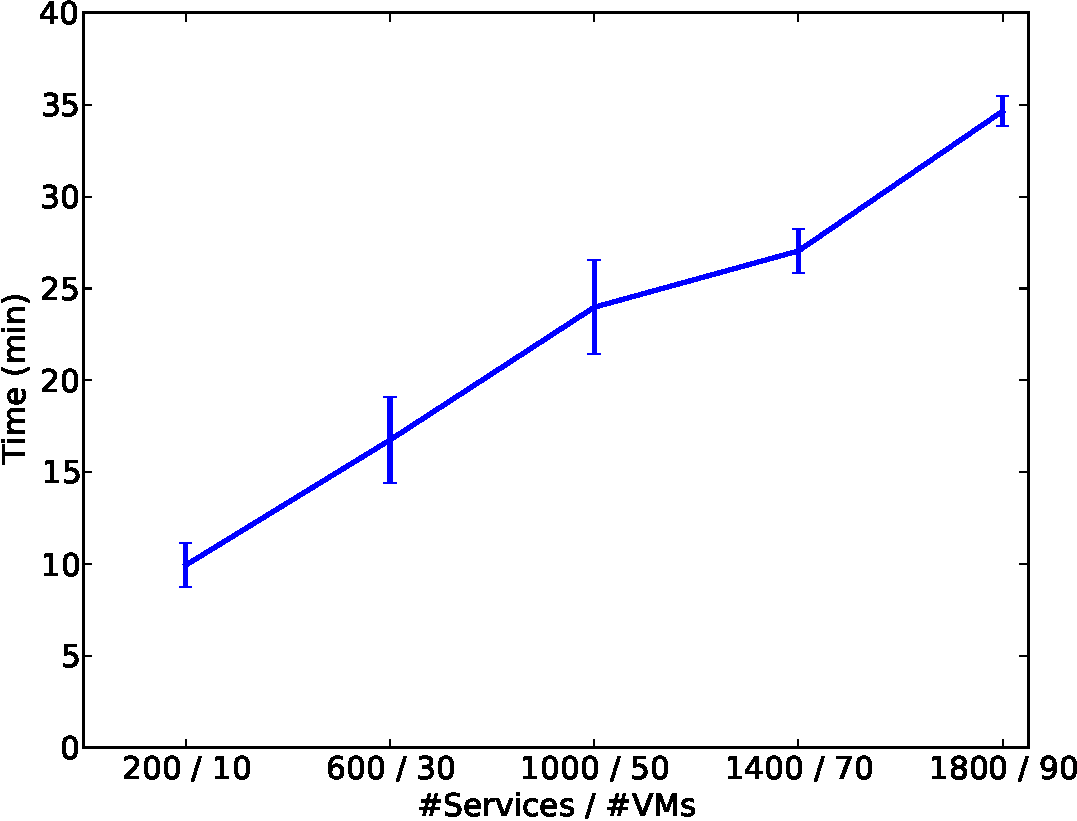
\includegraphics[width=.8\linewidth]{ee_scalability-crop.pdf}
  \caption{Average deployment times (with 95\% confidence interval) for increasingly larger compositions. The ratio between the number of services and the number of virtual machines is kept constant.}
  \label{fig:ee_scalability}
\end{figure}

These results show a good scalability in terms of deployed services.
Increasing 9 times the number of deployed services, the deployment time increased 3.5 times.
In absolute numbers, each increase in 400 deployed services 
was responsible for increasing the deployment time from 180 to 460 seconds. 
Note that even the highest time to deploy the service composition 
(about 35 minutes for 1,800 services) 
may be considered low if we consider the long period that 
such a large-scale composition is supposed to last until next update.

%%% Local Variables:
%%% mode: latex
%%% TeX-master: "ee_ccgrid.tex"
%%% End:
